\documentclass[12pt,letterpaper]{article}
\usepackage[utf8]{inputenc}
\usepackage{listings, float, xcolor}

%----- Configuración del estilo del documento------%
\usepackage{graphicx, fancyhdr, lastpage}
\usepackage{enumitem, pifont, hyperref, ulem}
\usepackage[left=2cm,right=2cm,top=1.8cm,bottom=2.3cm]{geometry}

\pagestyle{fancy}
\fancyhf{}
\rfoot{\textit{Página \thepage \hspace{1pt} de \pageref{LastPage}}}

%------ Paquetes matemáticos básicos --------%
\usepackage{amsmath, amssymb, amsthm}

%------ Personalizar el link al video  --------%
\hypersetup{
    colorlinks=true,
    linkcolor=blue!50!black, % Azul oscuro
    urlcolor=blue!50!black,  % Azul oscuro
    hidelinks % Elimina el recuadro azul
}

\begin{document}

%------ Encabezado -------- %
\begin{center}
\newcommand{\imp}{\rightarrow}
\newcommand{\vp}{\varphi}
  \begin{minipage}{3cm}
    \begin{center}
      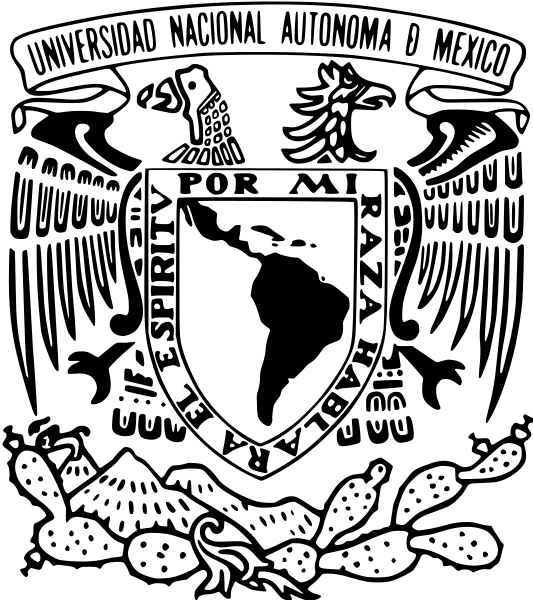
\includegraphics[height=3.4cm]{../unam_logo.png}
    \end{center}
  \end{minipage}\hfill
  \begin{minipage}{10cm}
    \begin{center}
      \textbf{\Large Universidad Nacional Autónoma de México}\\[0.2cm]
      \textbf{\large Facultad de Ciencias}\\[0.2cm]
      \textbf{Organización y Arquitectura de Computadoras 2025-2}\\[0.4cm]
      \textbf{\Large Práctica 05}\\[0.1cm]
      \textbf{Docentes:}\\
      José Galaviz \hspace{1em} Ricardo Pérez \hspace{1em} Ximena Lezama\\[0.3cm]
      \textbf{Autores:}\\
      Fernanda Ramírez Juárez \quad Ianluck Rojo Peña\\[0.3cm]
      \textbf{Fecha de entrega:} Jueves 20 de marzo de 2025
    \end{center}
  \end{minipage}\hfill
  \begin{minipage}{3cm}
    \begin{center}
      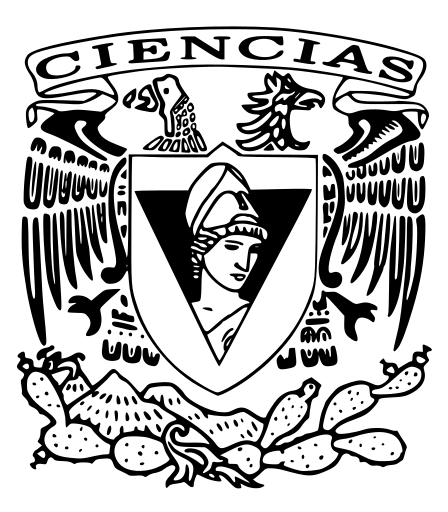
\includegraphics[height=3.4cm]{../fc_logo.png}
    \end{center}
  \end{minipage}
\end{center}

\bigskip
\hrule height 0.1pt
\bigskip

%------ Contenido -------- %
\section*{Ejercicios.}

\textbf{Mapas de Karnaugh para el Ejercicio 1.}
\begin{figure}[H]
  \centering
  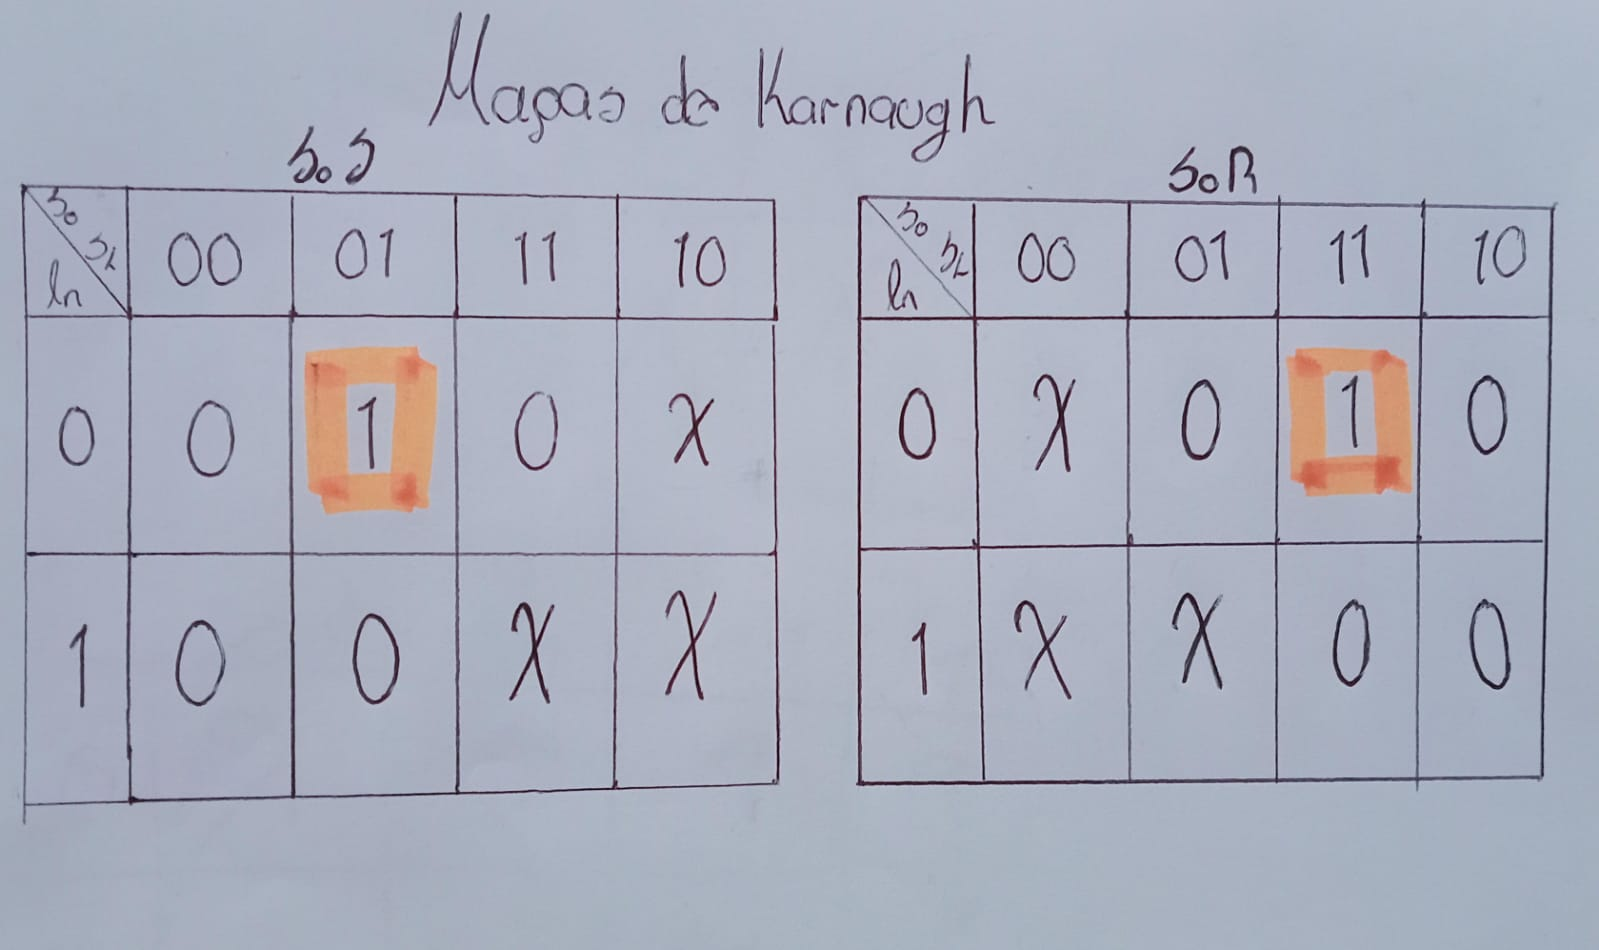
\includegraphics[width=0.6\textwidth]{karnaugh1.png}
\end{figure}

\begin{figure}[H]
  \centering
  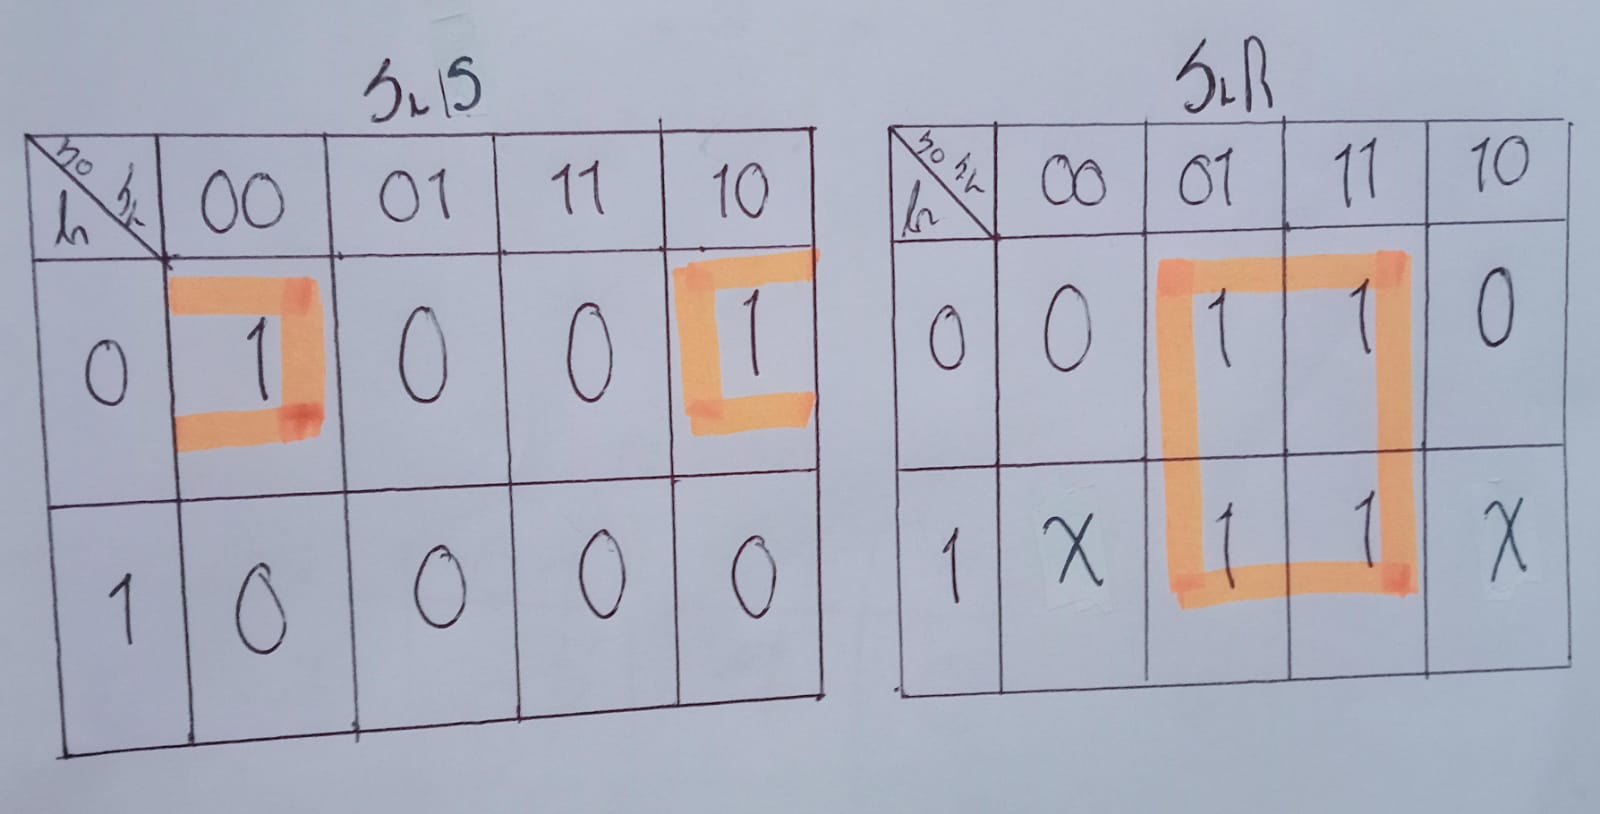
\includegraphics[width=0.6\textwidth]{Karnaugh2.png}
\end{figure}


\section*{Preguntas.}

\begin{enumerate}
\item En el contexto de los biestables: ¿Qué es el problema de la meta estabilidad? ¿Cómo puedes reducir la meta estabilidad en sistemas reales?
  \bigskip
  % -- Respuesta -- %
  
  Un biestable es un circuito multivibrador con dos estados estables, que puede cambiar de estado mediante señales de control. Su principal función es almacenar un bit de datos binarios y se emplea en aplicaciones como contadores, registros y divisores de frecuencia.\\
  La metaestabilidad ocurre cuando un biestable entra en un estado indefinido, la señal de entrada no cumple con los tiempos de establecimiento \textit{(setup time)} o retención \textit{(hold time)}, lo que impide que el biestable alcance un estado estable de manera confiable; almacenando un nivel lógico no válido. Este fenómeno puede manifestarse de dos formas:
  
  \textbf{Metaestabilidad analógica:} La salida se mantiene en un voltaje indefinido, cercano al umbral de conmutación.\\
  \textbf{Metaestabilidad oscilatoria:} La salida alterna repetidamente entre los dos niveles lógicos.
  
  La metaestabilidad puede provocar fallos en el funcionamiento del circuito digital y, en algunos casos, daños en el sistema. Su resolución es teóricamente ilimitada, dependiendo de la temporización de entrada y de ciertos parámetros del circuito.\\
  Si bien la metaestabilidad es inevitable en dispositivos biestables, se pueden implementar estrategias para mitigar sus efectos, tales como:

  \begin{itemize}
  \item \textbf{Uso de circuitos sincronizadores:}\\
    Consisten en biestables en cascada para filtrar estados metaestables antes de su uso en el sistema.
  \item \textbf{Circuitos de handshake:}\\
    Los cuales aseguran la correcta sincronización de señales asíncronas.
  \item \textbf{Sincronizadores de múltiples etapas con duplicadores de reloj:}\\
    Permiten estabilizar la señal de salida reduciendo el tiempo de resolución.
  \item \textbf{Selección de dispositivos con alto producto ganancia-ancho de banda:} \\
    Lo que minimizan el tiempo de recuperación del biestable.
  \item \textbf{Optimización del diseño del sistema:}\\
    Mantener una alimentación estable y controlar la temperatura del chip, ya que la degradación de la tensión de alimentación y el aumento de temperatura pueden agravar la metaestabilidad.
  \end{itemize}
  
  Estas medidas permiten mejorar la fiabilidad del sistema y reducir el impacto de la metaestabilidad en circuitos digitales críticos.
  
  \bigskip
  
\item ¿Qué es el \textbf{Sesgo de Reloj} (Clock Skew)? ¿Este fenómeno impacta la frecuencia máxima de un sistema?
    \bigskip
    % -- Respuesta -- % 

    El sesgo de reloj, o \textit{clock skew}, es la diferencia en el tiempo de llegada de la señal de reloj a registros secuenciales adyacentes dentro de un circuito síncrono, lo que provoca problemas de sincronización y afectar el rendimiento del sistema digital. Este desfase puede ser:
    
    \textbf{Positivo:} cuando la señal de reloj llega más tarde al registro receptor que al registro transmisor.\\
    \textbf{Negativo:} cuando la señal de reloj llega primero al registro receptor.
    
    Este fenómeno es un desafío crítico en el diseño digital, ya que puede provocar violaciones en las restricciones de temporización, afectando el correcto funcionamiento del circuito.\\
    El sesgo de reloj se origina principalmente por diferencias en el retraso de la red de distribución del reloj. Entre sus principales causas se incluyen:

    \begin{itemize}
    \item \textbf{Diferencias en Y = 2025- 1971 = la longitud de las interconexiones:}\\
      Si las rutas de entrega del reloj a registros secuenciales tienen longitudes distintas, la señal llegará en momentos diferentes.
      
    \item \textbf{Variaciones en los retardos de interconexión:}\\
      Factores como la resistencia, la capacitancia y el acoplamiento inductivo pueden generar diferencias de propagación en rutas de igual longitud.
      
    \item \textbf{Desigualdad en los retardos de las rutas lógicas:}\\
      La presencia de puertas lógicas en la distribución del reloj puede introducir retardos adicionales si no están balanceadas.
      
    \item \textbf{Factores ambientales y de fabricación:}\\
      Variaciones en la temperatura, diferencias en los procesos de fabricación e imperfecciones en los materiales pueden afectar la sincronización del reloj.
    \end{itemize}
    
    El sesgo de reloj influye directamente en la frecuencia máxima a la que puede operar un sistema. Un alto desfase puede reducir el margen de tiempo disponible para la propagación de datos entre registros, limitando la frecuencia de operación. Si el sesgo de reloj no se gestiona adecuadamente, puede llevar a fallos de temporización y errores en la ejecución del sistema digital.
    
    Para mitigar este efecto, se emplean técnicas como el \textbf{clock balancing} \textit{(equilibrio del reloj)}, el diseño simétrico de rutas de reloj y el uso de buffers para compensar diferencias de propagación.
    
    \bigskip
    
  \item ¿Qué es \textbf{Circuito Secuencial Tolerante a Fallos} (Fault Tolerant Sequential Circuit)? ¿Podemos hacer Tolerante a Fallos el Contador y el Banco de Registros que construimos?
    \bigskip
    % -- Respuesta -- %

    Un \textbf{Circuito Secuencial Tolerante a Fallos} es un tipo de circuito digital diseñado específicamente para seguir funcionando correctamente incluso cuando ocurren errores o fallas en alguno de sus componentes. En como un sistema que puede \textit{sobrevivir} a los problemas y continuar realizando sus tareas sin interrupcion graves.\\
    Existen varias técnicas para lograr la tolerancia a fallos en circuitos secuenciales, algunas de las más comunes son:

    \begin{itemize}
    \item \textbf{Redundancia de Hardware:}\\
      Esta técnica implica duplicar o triplicar los componentes críticos del circuito. Si un componente falla, los otros pueden tomar el control y mantener el sistema en funcionamiento.
      
    \item \textbf{Detección y Corrección de Errores:}\\
      Se utilizan códigos especiales y circuitos adicionales para detectar errores en los datos y corregirlos automáticamente. Esto asegura que la información procesada por el circuito sea precisa y confiable.
      
    \item \textbf{Reconfiguración Dinámica:}\\
      En sistemas más avanzados, el circuito puede reconfigurarse automáticamente para evitar componentes defectuosos. Si se detecta una falla, el sistema puede cambiar su configuración para utilizar componentes alternativos.
      
    \item \textbf{Recuperación de fallos:}\\
      Esta técnica consiste en que el sistema pueda regresar a un estado de operación estable y correcto, despues de que ocurra una falla.
    \end{itemize}
    
    Estos circuitos son esenciales en una amplia gama de aplicaciones críticas, incluyendo:
    \begin{itemize}
    \item \textbf{Sistemas aeroespaciales:}\\
      Aviones, satélites y naves espaciales.
    \item \textbf{Equipos médicos:}\\
      Dispositivos de monitoreo, máquinas de diagnóstico y sistemas de soporte vital.
    \item \textbf{Sistemas de control industrial:}\\
      Plantas de energía, fábricas y sistemas de transporte.
    \item \textbf{Sistemas de telecomunicaciones:}\\
      Redes de comunicación y equipos de transmisión.
    \item \textbf{Sistemas informáticos críticos:}\\
      Servidores, sistemas de almacenamiento de datos y aplicaciones financieras
    \end{itemize}

    Y sí, sí es posible implementar tolerancia a fallos tanto en el banco de registros como en el contador.
    
    En el caso del contador, al ser un circuito secuencial que sigue una secuencia lógica predefinida, será relativamente sencillo detectar errores si su valor se desvía del patrón esperado. Para ello podemos:

    \begin{itemize}
    \item Implementar múltiples contadores en paralelo y comparar sus resultados para detectar discrepancias.
    \item Incorporar circuitos adicionales que validen la transición correcta entre estados.
    \end{itemize}
    
    Por otro lado, el banco de registros, lo podemos hacer tolerante a fallos implementando:
    
    \begin{itemize}
      \item Mantener múltiples copias de cada valor almacenado para su recuperación en caso de error.
      \item Bits adicionales para corrección de errores.
      \item Verificación de coherencia.
\end{itemize}
    \bigskip
    
  \item Existen 2 tipos de maquinas de estado finito que usan Flip-Flops. ¿Cuáles son?¿En qué se diferencian?
    \bigskip
    % -- Respuesta -- %

    Las máquinas de estado finito que utilizan flip-flops se dividen:
    
    \begin{enumerate}[label=\arabic*)]
    \item \textbf{Máquina de Mealy.}

      \begin{itemize}
      \item La salida depende tanto del estado actual como de las entradas actuales.
      \item Su circuito combinacional genera la salida considerando el estado y las entradas en ese instante.
      \item Dado que las salidas pueden cambiar en respuesta inmediata a una entrada, las máquinas de Mealy suelen reaccionar más rápido a cambios en la entrada.
      \item En su representación gráfica, las salidas se escriben en las transiciones entre estados, junto con las entradas correspondientes.
      \end{itemize}

      \begin{figure}[H]
        \centering
        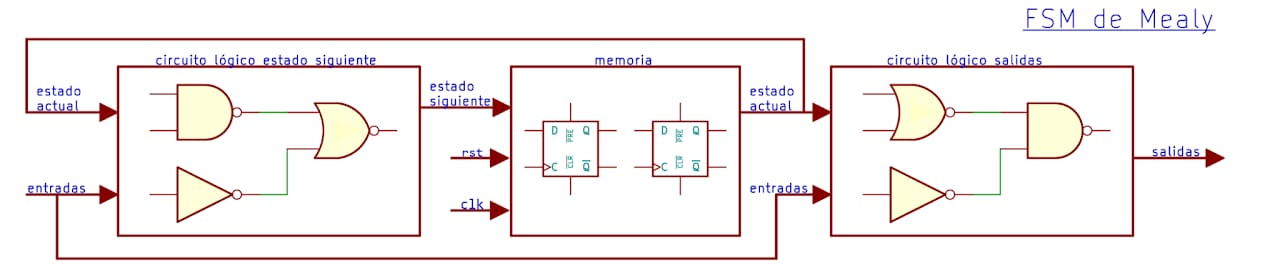
\includegraphics[width=1.1\textwidth]{imagen2.png}
      \end{figure}
      
    \item \textbf{Máquina de Moore.}
      \begin{itemize}
      \item La salida depende únicamente del estado actual, sin considerar las entradas directamente.
      \item El circuito combinacional que genera la salida solo toma en cuenta el estado de la máquina.
      \item Generalmente requiere más estados que una máquina de Mealy equivalente, ya que cada estado debe reflejar las posibles salidas.
      \item En su representación, la salida se asocia al estado mismo, mientras que las entradas se indican en las transiciones.
      \end{itemize}

      \begin{figure}[H]
        \centering
        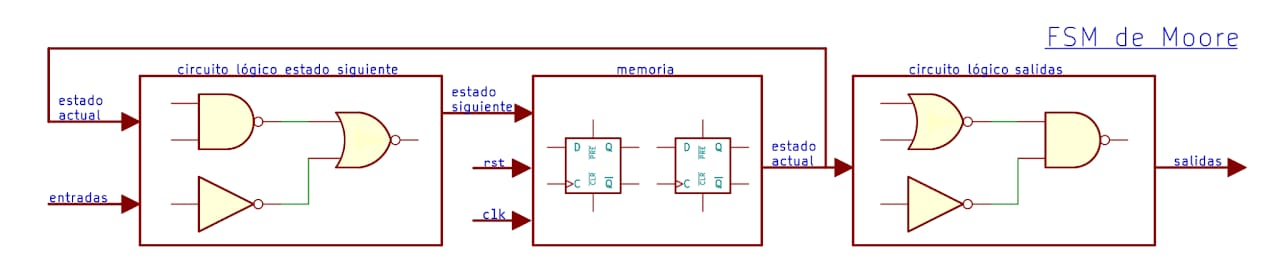
\includegraphics[width=1.1\textwidth]{imagen1.png}
      \end{figure}
    \end{enumerate}

    La principal diferencia radica en cómo se determinan las salidas:\\
    En una máquina de Mealy, la salida cambia inmediatamente en función de la entrada y el estado.\\
    En una máquina de Moore, la salida solo cambia cuando el estado se actualiza.\\
    Debido a estas diferencias, las máquinas de Mealy pueden ser más rápidas en respuesta, mientras que las máquinas de Moore ofrecen mayor estabilidad en las salidas, evitando cambios bruscos ante variaciones momentáneas en la entrada.
    
    \begin{figure}[H]
      \centering
      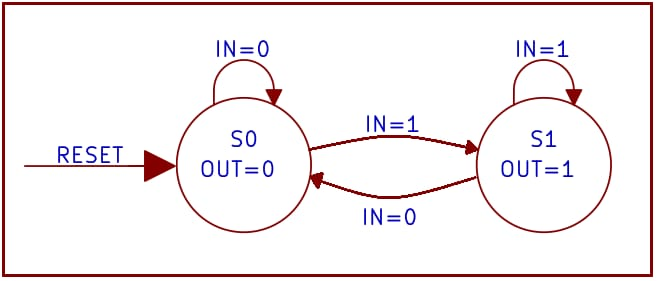
\includegraphics[width=0.7\textwidth]{imagen3.png}
    \end{figure}
    
    \begin{figure}[H]
      \centering
      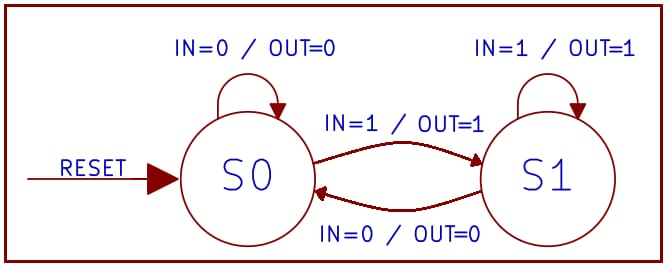
\includegraphics[width=0.7\textwidth]{imagen4.png}
    \end{figure}
\end{enumerate}

\section*{Punto Extra.}
Link al video para el punto extra:
\href{https://drive.google.com/file/d/1H5akXyFdoc_lS8LiLSPnFHDVVvcUcsfj/view?usp=drivesdk}{\textit{\uline{Registro de 4 bits con Latch tipo D}}}
\end{document}
